In the previous sections, all of our considerations depended upon the existence of a conserved negative and ``global'' (as seen by a static observer at infinity) energy. This is only possible if the spacetime under consideration is stationary. 

In this section we will demonstrate how one can still observe the PP even in cases where this assumption is relaxed and there is no global and conserved energy available to be explored, thus, looking only at locally defined quantities. This technique allows one to study the Penrose mechanism even when the spacetime metric is defined numerically, such as is the case in numerical simulations of binary black hole collisions.

\subsection{3+1 split of the geodesic equation}

To understand our proposed technique, it is first fundamental to understand how General Relativity can be reformulated by explicitly separating its spatial and temporal components. This decomposition know as a ``3+1 split'' is very commonly used in Numerical Relativity and was motivated by the first attempts of posing GR as a Cauchy problem. Numerical Relativity codes very often provide ways to access the spacetime metrics being evolved in terms of its 3+1 components.

In this section, we will assume familiarity of the reader with this concept which can be readily reviewed in Refs.~\cite{Alcubierre2012-xp, 9780521514071, 9781108928250}. Given that the PP requires us to investigate the trajectories of particles in a background spacetime, we must now solve the geodesic equation taking into account that the spacetime metric (and its derivatives) will be provided via 3+1 split components. 

The need to solve the geodesic equation in this context overlaps with works that are interested in simulating an image of a black hole, that is, determining what a camera would capture if it was pointed towards a black hole. In this type of simulation a technique called \emph{backwards ray tracing} is employed, which consists in choosing a position and orientation of a model camera and integrating the trajectory of the photons that hit the camera's ``film'' backwards in time. In the event that the photon is assimilated by the system, the corresponding pixel within the image will appear black. If the photon ``collides'' with an obstacle such as a distant star or even an artificially colored background, the hue of the pixel is equivalent to the hue of that specific obstacle.

In spite of divergent objectives, the mathematical instruments utilized in backwards ray tracing are integral to the procedure that will imminently be formulated. The exhaustive and intricate derivation of the 3+1 decomposition of the geodesic equation utilized in this segment can be located in Ref.~\cite{Vincent_2012}. The terminologies and notions that are required for the development of our proposal will be derived from this source. 

Initially, we consider a globally hyperbolic spacetime that can be characterized by a metric tensor $\mtrtens{\mu}{\nu}$. Since it is globally hyperbolic, it allows for a foliation of constant coordinate time $t$ hypersurfaces that can be specified as $\Sigma_t$. We shall assume that the spacetime is equipped with coordinates\footnote{Our convention entails that Greek indices encompass all four coordinates, whereas Latin indices include only spatial coordinates.} that are adapted to the foliation, such that $x^0=t$ and $x^i$ ranges over $\Sigma_t$.

The unit time-like (directed towards the future) normal vector of $\Sigma_t$ shall be identified as $n^\mu$. This vector coincides with the four-velocity of an observer, known as the \emph{Eulerian Observer} or $\mathcal{O}E$, whose worldlines are orthogonal to $\Sigma_t$. The spatial metric induced in $\Sigma_t$ is designated as $\gamma{\mu\nu}$, and its associated covariant derivative is $D_i$. The extrinsic curvature tensor is $K_{ij}$, the lapse function is $N$, and the shift vector is $\beta^\mu$. The line element of the $3+1$ decompose metric then becomes
%
\begin{equation}
  \ud s^2 = -N^2 \ud t^2 + \gamma_{ij}(\ud x^i + \beta^i \ud t)(\ud x^j + \beta^j \ud t).
  \label{eq:arbitrary_penrose_decomposed_metric}
\end{equation}

Let us now consider a particle $\mathcal{P}$ of 4-momentum $p^\mu$. Let us assume that the particle moves in either a time-like or null geodesic (and thus without the influence of any force but gravity), which implies that
%
\begin{equation}
  p_\mu p^\mu = m^2\delta,
  \label{eq:arbitrary_penrose_p_norm}
\end{equation}
% 
where $\delta = -1$ for massive particles (and in this case $m$ represents the particle's mass) or $\delta=0$ for photons. The 4-momentum can be decomposed as
%
\begin{equation}
  p^\mu = E(n^\mu + V^\mu)
  \label{eq:arbitrary_penrose_p_decomp}
\end{equation}
%
where $E$ represents the particle's energy as measured by $\mathcal{O}_E$ (by definition,  $E = - n_\mu p^\mu$) and $V^\mu$ represents the 3-velocity of the particle, also as measured by $\mathcal{O}_E$. The 3-momentum $P^\mu$ of $\mathcal{P}$ as observed by $\mathcal{O}_E$ is thus
%
\begin{equation}
  P^\mu \equiv \tens{\gamma}{\mu}{\nu} p^\nu = E V^\mu.
  \label{eq:arbitrary_penrose_3_momentum}
\end{equation}
%
The normalization of $p^\mu$ and $n_\mu$, together with the orthogonality relation $n_\mu V^\mu = 0$ and Eq.~\eqref{eq:arbitrary_penrose_p_decomp} imposes
%
\begin{equation}
  V_\mu V^\mu = V_i V^i  = 1 + \delta\left(\frac{m}{E}\right)^2.
  \label{eq:arbitrary_penrose_V_norm}
\end{equation}
%
Finally, parametrizing the particle's position vector $X^i$ by the coordinate time (that is $x^i = X^i(t)$) the geodesic equation of $\mathcal{P}$ is decomposed in a set of 7 equations, namely
%
\begin{align}
  \der{X^i}{t} & = N V^i - \beta^i \label{eq:arbitrary_penrose_geodesic_eq_X}                                                                                                                                                  \\
  \der{V^i}{t} & = N V^j\left[ V^i \left( \partial_j \ln N - K_{jk} V^k \right) + 2 \tens{K}{i}{j} - {}^3\Gamma^{i}_{jk}V^k\right] - \gamma^{ij}\partial_j N - V^j\partial_j\beta^i \label{eq:arbitrary_penrose_geodesic_eq_V} \\
  \der{E}{t}   & = E (N K_{jk} V^j V^k - V^j \partial_j N) \label{eq:arbitrary_penrose_geodesic_eq_E}
\end{align}
%
where ${}^3\Gamma^{i}_{jk}$ are the Christoffel symbols associated with $\gamma_{ij}$.

\subsection{Penrose process}

Henceforth, $E$ shall be designated as the \emph{local energy}, given that it is gauged locally by the observer that is orthogonal to the foliation (the Eulerian Observer). In Sections~\ref{ch:penrose_binaries:sec:penrose_review}-\ref{ch:penrose_binaries:sec:cmmr_penrose}, we have been addressing what shall henceforth be referred to as the \emph{global energy}, i.e., the energy measured by a static observer stationed at infinity, which we shall now denote by $\varepsilon$. Our investigation necessitates the establishment of a connection between these two quantities, and we shall proceed to do so at this point. The global energy, $\varepsilon$ is defined as
%
\begin{equation}
  \varepsilon = - p_\mu \xi^\mu.
  \label{eq:arbitrary_penrose_global_energy_def}
\end{equation}
%
where $\xi^\mu = (\partial_t)^\mu$.
%
Expanding the contraction in Eq.~\eqref{eq:arbitrary_penrose_global_energy_def} with the general metric given in Eq.~\eqref{eq:arbitrary_penrose_decomposed_metric} and with the 4-momentum given in Eq.~\eqref{eq:arbitrary_penrose_p_decomp}, we get
%
\begin{equation}
  \varepsilon = \left( N - \gamma_{ij} \beta^i V^j \right) E.
  \label{eq:arbitrary_penrose_local_global_energy_relation}
\end{equation}

It is noteworthy that in the event that $\xi^\mu$ denotes a global time-like killing vector field pertaining to the background spacetime metric, $\varepsilon$ emerges as a conserved quantity along a particle's trajectory. As previously demonstrated, this fact was utilized to determine whether energy was extracted as an outcome of a particle disintegration process by evaluating the global energies of the particles implicated, one of which was necessarily characterized by a negative energy value. Due to the invariance of $\varepsilon$ along the particle's trajectories, the timing and location of this comparison were irrelevant.

If we, however, relax the assumption that the $\xi^\mu$ is a global time-like killing vector field, the quantity given by Eq.~\eqref{eq:arbitrary_penrose_global_energy_def} is no longer physically meaningful as an energy measure, thus restricting all physical arguments to be made in terms of local energy $E$ measurements. Furthermore, local energy, as can be explicitly seen in Eq.~\eqref{eq:arbitrary_penrose_geodesic_eq_E}, is not in general conserved along the particle's trajectory and must always be positive in order to be physically meaningful.

Given the aforementioned constraints, how can the local energies of particles engaged in a collision or a breakup process be compared in a physically significant manner to determine whether the system has lost or gained energy? To resolve this issue, it is essential to consider a crucial implication of Eq.~\eqref{eq:arbitrary_penrose_local_global_energy_relation}, which is that if the spacetime metric is asymptotically flat, meaning it becomes the Minkowski solution at an infinitely remote distance from the black hole (or holes), a significant inference can be derived.

In the limit where spatial coordinates approach infinity, the components of the spatial metric $\gamma_{ij}$ approach those of the Minkowski metric $\eta_{ij}$, the shift vector $\beta^i$ approaches zero, and the lapse function $N$ approaches one. Therefore, according to Eq.~\eqref{eq:arbitrary_penrose_local_global_energy_relation}, the global energy $\varepsilon$ and the local energy $E$ coincide at infinity. This means that if the spacetime is asymptotically flat, the global energy is still physically meaningful at infinity. Moreover, Eq.~\eqref{eq:arbitrary_penrose_geodesic_eq_E} implies that $K_{ij}$ approaches zero and $N$ approaches one as the Minkowski solution is approached, so both global and local energies are conserved at infinity.

In practical terms (and especially when analyzing spacetime metrics obtained from numerical simulation codes) it is not possible to integrate a trajectory to spatial infinity since the coordinates commonly employed are not compactified and such compactification schemes are often difficult or impossible to perform in practice.

Instead of attempting to do so, our technique follows again a practice common in backward ray tracing works, more specifically, we follow the prescription given by Ref.~\cite{Bohn:2014xxa}. Given a set of initial conditions $X^i(0), V^i(0), E(0)$, we evolve the system formed by Eqs.~\eqref{eq:arbitrary_penrose_geodesic_eq_X}-\eqref{eq:arbitrary_penrose_geodesic_eq_E} numerically until the particle reaches a sphere of predetermined radius that we denominate the \emph{background sphere}. The radius of this sphere is chosen so that the difference between global and local energy becomes smaller than a certain threshold $\delta_E$, that is, 
%
\begin{equation}
  |E(t_f)- \varepsilon(t_f)| < \delta_E,
  \label{eq:arbitrary_penrose_background_sphere_cplision_condition}
\end{equation}
%
where $t_f$ represents the final integration coordinate time. Additionally, we also stop integrating if the particle is absorbed by the system at a given time of ``swallowing'' $t_S$. A particle is considered absorbed if the difference of its local energy at $t_S$ and at $t=0$ gets larger than a certain swallowing threshold $\delta_S$, that is, 
%
\begin{equation}
  |E(t_S) - E(0)|/E(0) = \delta_S.
  \label{eq:arbitrary_penrose_swallowing_condition}
\end{equation}

The scheme described above was implemented in a public \texttt{C++} code available in Ref.~\cite{GRLensingRepo}. Compilation and usage instructions are provided within the repository. See Appendix~\ref{app:grlensing} for further information.

\subsection{Parametrizing initial velocities}

As previously stated, the initial configuration of particles is determined by seven parameters: the initial positions $X^i(0)$, velocities $V^i(0)$, and local energy $E(0)$. Upon selecting a breakup point and initial energy, the task of determining the remaining three initial velocities persists. It is important to recall that the initial data must fulfill Eq.~\eqref{eq:arbitrary_penrose_V_norm}. Therefore, for generic $V^i(0)$ and $E(0)$ values and considering massive particles, we can write
%
\begin{multline}
  \gamma_{ij} V^{i}(0)V^{j}(0) = \gamma_{11}\left(V^1(0)\right)^2 + \gamma_{22}\left(V^2(0)\right)^2 + \gamma_{33}\left(V^3(0)\right)^2 \\
  + 2\left[ \gamma_{12}V^1(0)V^2(0) + \gamma_{13}V^1(0)V^3(0) + \gamma_{23}V^2(0)V^3(0) \right] = 1-\left(\frac{m}{E(0)}\right)^2.
  \label{eq:arbitrary_penrose_initial_v_explicit_expansion}
\end{multline}

Equation \eqref{eq:arbitrary_penrose_initial_v_explicit_expansion} can be identified as a quadratic form with three variables, $V^i(0)$. For the purpose of our study, we will only consider particles that are initially confined to the $z=0$ plane of the system, which means selecting $V^z(0) = 0$. This choice significantly simplifies the mathematical analysis of the initial conditions, enabling us to associate Eq.~\eqref{eq:arbitrary_penrose_initial_v_explicit_expansion} with the general bi-variate quadratic form
%
\begin{equation}
  A X^2 + 2 B X Y + C Y^2 + 2 D X + 2 F Y + G = 0,
  \label{eq:arbitrary_penrose_general_quadratic_form}
\end{equation}
%
where
%
\begin{align}
  A & = \gamma_{11},                                      \\
  B & = \gamma_{12},                                      \\
  C & = \gamma_{22},                                      \\
  G & = -\left[ 1 - \left( \frac{m}{E} \right)^2 \right], \\
  D & = F = 0,
\end{align}
%
and
%
\begin{align}
  X & = V^1(0),  \\
  Y & = V^2(0).
\end{align}

Let us define the determinants $\Delta$, $J$ and $I$ as
%
\begin{equation}
  \Delta = 
  \begin{vmatrix}
    A & B & D  \\
    B & C & F  \\
    D & F & G
  \end{vmatrix}
  = \left( 1 - \left( \frac{m}{E} \right)^2 \right) \left(\gamma_{12}^2-\gamma_{11} \gamma_{22}\right)
  \label{eq:arbitrary_penrose_quadratic_determinant}
  ,
\end{equation}
%
\begin{equation}
  J = 
  \begin{vmatrix}
    A & B \\
    B & C \\
  \end{vmatrix}
  = -gamma_{12}^2 + \gamma_{11}\gamma{22}
  \label{eq:arbitrary_penrose_quadratic_J}
\end{equation}
%
and
%
\begin{equation}
  I = A + C = \gamma_{11} + \gamma_{22}.
  \label{eq:arbitrary_penrose_quadratic_I}
\end{equation}

If one has
%
\begin{align}
  \Delta \neq 0, \\
  J > 0,         \\
  \Delta / I < 0,
\end{align}
%
the quadratic of Eq.~\eqref{eq:arbitrary_penrose_general_quadratic_form} describes a non-degenerate real ellipse in the $V^1(0)$-$V^2(0)$ plane~\cite{Hart2002}. The center coordinates of this ellipse will be denoted as $V^1(0)_\circ$ and $V^2(0)_\circ$, while the lengths of its semi-major and semi-minor axes will be represented as $\alpha_+$ and $\alpha_-$, respectively. Additionally, the angle of rotation, which is measured counterclockwise from the $V^1$ axis to the semi-major axis $\alpha_+$, will be designated as $\phi$. From the coefficients of the quadratic, we can then explicitly write~\cite{Larson2006, Young2010, Lawrence2014}
%
\begin{equation}
  V^1_\circ = V^2_\circ = 0,
  \label{eq:arbitrary_penrose_ellipse_centers}
\end{equation}
%
\begin{equation}
  \alpha_\pm = \sqrt{ \frac{2 \left( 1 - \left(m/E\right)^2 \right)}{\gamma_{11} \mp \sqrt{4 \gamma_{12}^2 + \left( \gamma_{11} - \gamma_{22} \right)^2} +\gamma_{22}} }
  \label{eq:arbitrary_penrose_ellipse_axis}
\end{equation}
%
and
\begin{equation}
  \phi =
  \begin{cases}
    0                                                                                                 & \text{if } \gamma_{12} = 0 \text{ and } \gamma_{11} < \gamma_{22}    \\
    \frac{\pi}{2}                                                                                     & \text{if } \gamma_{12} = 0 \text{ and } \gamma_{11} > \gamma_{22}    \\
    \frac{1}{2} \cot^{-1} \left( \frac{\gamma_{11}-\gamma_{22}}{2\gamma_{12}} \right)                 & \text{if } \gamma_{12} \neq 0 \text{ and } \gamma_{11} < \gamma_{22} \\
    \frac{\pi}{2} + \frac{1}{2} \cot^{-1} \left( \frac{\gamma_{11}-\gamma_{22}}{2\gamma_{12}} \right) & \text{if } \gamma_{12} \neq 0 \text{ and } \gamma_{11} > \gamma_{22}
  \end{cases}
  .
  \label{eq:arbitrary_penrose_ellipse_angle}
\end{equation}

With these quantities, it is possible to describe the ellipse in terms of an arbitrary parameter $\Theta \in \left[0,2\pi\right]$, that is,
%
\begin{align}
  V^{1}_{\Theta}(0) & =  V^{1}_\circ + \alpha_{+} \cos\Theta\cos\phi - \alpha_{-}\sin\Theta\sin\phi                                                  \label{eq:arbitrary_penrose_ellipse_parametric_1} \\
  V^{2}_{\Theta}(0) & = V^{2}_\circ + \alpha_{-} \sin\Theta\cos\phi + \alpha_{+}\cos\Theta\sin\phi, \label{eq:arbitrary_penrose_ellipse_parametric_2}
\end{align}
%
and thus the problem of finding initial velocities that satisfy Eq.~\eqref{eq:arbitrary_penrose_V_norm} is reduced to that of evaluating the right-hand side of Eqs.~\eqref{eq:arbitrary_penrose_ellipse_parametric_1} - \eqref{eq:arbitrary_penrose_ellipse_parametric_2} for some value of $\Theta$, effectively reducing the degrees of freedom of the problem.

Utilizing this parametrization of velocities, the general workflow for finding explicit examples of the PP with our code is as follows:

\begin{enumerate}
  \item Chose a break-up point. This will be the initial position of all three particle participating in the process. We know that in order to extract energy this break-up must occur inside the ergosphere. In general, when the spacetime under study does not possess a global time-like killing vector field, we consider the ergosphere to be the now observer dependent region where the metric component $\mtrtens{t}{t}$ changes sign.
  \item Chose initial velocities and energy for the ingoing particle in such a way that it is an escaping orbit when integrated forward and backward in time. Requiring that the orbit is escaping in both ``temporal directions'' makes it more likely that one of the particles produced after the break-up will escape to infinity.
  \item Choose initial velocities and energy for the particle that is absorbed by the black whole and will be the equivalent of the negative energy orbit. These parameters are chosen so that the particle is counter-rotating with the black whole that will absorb it, so that its angular momentum can actually be decreased upon absorption.
  \item The escape orbit parameters are computed automatically by the code via 4-momentum conservation at the break-up point.
\end{enumerate}

\subsection{Kerr Metric}
\label{ch:kerr_example}
As an illustrative example and proof of concept, we will demonstrate the procedure described so far applied to the Kerr metric. In Kerr-Schild coordinates $(t,x,y,z)$, the metric components are given by~\cite{PhysRevD.66.084024}
%
\begin{equation}
  \mtrtens{\mu}{\nu} = \eta_{\mu \nu} + 2 H l_\mu l_\nu,
  \label{eq:arbitrary_penrose_kerr_ks_line_element}
\end{equation}
%
where
%
\begin{equation}
  H = \frac{M r^3}{r^4 + a^2 z^2},
  \label{eq:arbitrary_penrose_kerr_ks_H}
\end{equation}
%
\begin{equation}
  l_\mu = \left( 1, \frac{rx + ay}{r^2 + a^2}, \frac{ry - ax}{r^2 + a^2}, \frac{z}{r} \right),
  \label{eq:arbitrary_penrose_kerr_ks_l}
\end{equation}
%
\begin{equation}
  r^2 = \frac{1}{2}\left( \rho^2 - a^2 \right) + \sqrt{\frac{1}{4} \left( \rho^2 - a^2 \right)^2 + a^2z^2},
  \label{eq:arbitrary_penrose_kerr_ks_r}
\end{equation}
%
$M$ is the black hole mass, $a$ its spin parameter and $\rho = \sqrt{x^2 + y^2 + z^2}$.

By comparison with Eq.~\eqref{eq:arbitrary_penrose_decomposed_metric} it is easy to identify the metric's ADM components. The lapse is given by~\cite{PhysRevD.66.084024}
%
\begin{equation}
  N = \frac{1}{\sqrt{1 + 2 H}},
  \label{eq:arbitrary_penrose_kerr_ks_lapse}
\end{equation}
%
the sift vectors are
%
\begin{align}
  \beta_i & = 2 H l_i \label{eq:arbitrary_penrose_kerr_ks_l_shift}                                                      \\
  \beta^i & = \frac{2 H \tens{\delta}{ij}{} l_j }{\left( 1 + 2 H \right)}, \label{eq:arbitrary_penrose_kerr_ks_u_shift}
\end{align}
%
the 3-metric is
%
\begin{equation}
  \gamma_{ij} = \eta_{ij} + 2 H l_i l_j
  \label{eq:arbitrary_penrose_kerr_ks_3_metric}
\end{equation}
%
and the extrinsic curvature is
%
\begin{equation}
  K_{ij} = -\indexdel{t}\left( H l_i l_j \right)/N + 2 \left( D_i \left( H l_j \right) + D_j \left( H l_i \right) \right)
  \label{eq:arbitrary_penrose_kerr_ks_3_extrinsic_curvature}
\end{equation}
%
where $D_i$ is the covariant derivative associated with $\gamma_{ij}$.

We will now summarize the parameter choices made that provide an explicit example of energy extraction. In this example, we have chosen $M = 0.5$ and $a = 0.49$, which is equivalent to 98\% of $M$, a rather large spin parameter, chosen to facilitate the process of finding suitable orbits. The break-up point was chosen at coordinates $X^i = (1, 0, 0)$ and the background sphere radius was chosen to be $1.0\times 10^6$. Table~\ref{tab:arbitrary_penrose_kerr_example_energy_mass} summarizes the initial energy and mass of the participating particles. The first, second and third rows contain data relative to the entry, Penrose and exit orbits, respectively. The parameters for the entry and Penrose orbits are chosen explicitly via configuration file fed to the code, while the parameters of the exit orbit are computed via the conservation of 4-momentum at the break-point. Note that the masses are explicitly chosen in order to satisfy Eq.~\eqref{eq:mass_constraint} and to provide a way of computing initial velocities via Eqs.~\eqref{eq:arbitrary_penrose_ellipse_parametric_1}-\eqref{eq:arbitrary_penrose_ellipse_parametric_2}

\begin{table}[]
  \centering
  \begin{tabular}{cc}
    \hline\hline
    $E(0)$                              & $m$                                 \\
    $1.0$                               & $1.0 \times 10^{-1}$                \\
    $8.0 \times 10^{-3}$                & $1.0 \times 10^{-4}$                \\
    $9.9199999999999999 \times 10^{-1}$ & $9.5800493929138735 \times 10^{-3}$ \\ \hline\hline
  \end{tabular}
  \caption{Initial energy and masses for the particles participating in the Penrose process example. The first two rows are given explicitly via configuration value and represent the ingoing and Penrose trajectories, respectively. The third row represents the exit trajectory and is computes via conservation of 4-momentum.}
  \label{tab:arbitrary_penrose_kerr_example_energy_mass}
\end{table}

Table~\ref{tab:arbitrary_penrose_kerr_example_velocities} summarize the initial velocities of the participating particles. Here, the values of the first two rows (representing the ingoing and Penrose trajectories, respectively), were computed via the parametrization described in the previous section together with data from Tab.~\ref{tab:arbitrary_penrose_kerr_example_energy_mass} while data on the third row, representing the outgoing particle, was computed via conservation of 4-momentum. The third column in this table shows the value of the ellipse parameter chosen for each orbit (except the exit orbit).

\begin{table}[]
  \centering
  \begin{tabular}{ccc}
    \hline\hline
    $V^x(0)$              & $V^y(0)$              & $\Theta$       \\
    $0.6769503786998466$  & $0.6740022058848380$  & $-25/200 \pi$  \\
    $0.5948571400034293$  & $-0.3343724878526367$ & $-100/200 \pi$ \\
    $0.67761242094739838$ & $0.68213425986659171$ & ---            \\ \hline\hline
  \end{tabular}
  \caption{Initial velocities for the particles participating in the Penrose process example. The first two rows are computed using the ellipse parametrization described in the previous section with data provided in Tab.~\ref{tab:arbitrary_penrose_kerr_example_energy_mass} together with the parameter provided in the third column and represent the ingoing and Penrose trajectories, respectively. The third row represents the exit trajectory and is computes via conservation of 4-momentum.}
  \label{tab:arbitrary_penrose_kerr_example_velocities}
\end{table}

Table~\ref{tab:arbitrary_penrose_kerr_example_results} summarizes the two energy measures (local and global on the first and second column, respectively) at the time when they hit the background sphere. The first row contains data relative to the ingoing orbit while the second contains data relative to the outgoing orbit. Note that $t_f$ does not necessarily coincide for the two orbits, since they might take arbitrarily long paths before escaping to infinity. The third column shows the absolute difference between global and local energies at the background sphere.

\begin{table}[]
  \centering
  \resizebox{\textwidth}{!}{
    \begin{tabular}{ccc}
      \hline\hline
      $E(t_f)$                            & $\varepsilon(t_f)$                  & $|E(t_f) - \varepsilon(t_f)|$       \\
      $3.8435595988010596 \times 10^{-1}$ & $3.8435613882134312 \times 10^{-1}$ & $1.7894123710560095 \times 10^{-7}$ \\
      $3.8515962539170862 \times 10^{-1}$ & $3.8515904777176790 \times 10^{-1}$ & $5.776199407114824 \times 10^{-7}$  \\ \hline\hline
    \end{tabular}
  }
  \caption{Energy measures at the time of collision with the background sphere. The first and second row represent the ingoing and the outgoing orbits, respectively. The third column shows the absolute difference between energy measures at the background sphere radius. Note that $t_f$ is not necessarily the same for both trajectories.}
  \label{tab:arbitrary_penrose_kerr_example_results}
\end{table}

Finally, Table~\ref{tab:arbitrary_penrose_kerr_example_efficiency} summarizes the amount of energy extracted from the process in different forms. The first and second rows compute the difference between the energy of the outgoing and ingoing particles using different energy measures (local and global respectively). Since this difference is positive, we can conclude that energy was indeed extracted from the black hole. The last two rows compute the efficiency of the process for the two available energy measures. The efficiency of the process for a given energy measure $\epsilon$ is given by
%
\begin{equation}
  \eta_\epsilon = \frac{\epsilon_\text{out}(t_f) - \epsilon_\text{in}(t_f)}{\epsilon_\text{in}(t_f)}.
  \label{eq:arbitrary_penrose_kerr_example_efficiency_formula}
\end{equation}

\begin{table}[]
  \centering
  \begin{tabular}{cc}
    \hline\hline
    $E_\text{out}(t_f)-E_\text{in}(t_f)$                     & $0.0008036655116026026$ \\
    $\varepsilon_\text{out}(t_f)-\varepsilon_\text{in}(t_f)$ & $0.0008029089504247855$ \\
    $\eta_E$                                                 & $0.0020909406786700896$ \\
    $\eta_\varepsilon$                                       & $0.0020889722919224165$ \\ \hline\hline
  \end{tabular}
  \caption{Energy difference and extraction efficiency of the process given different energy measures.}
  \label{tab:arbitrary_penrose_kerr_example_efficiency}
\end{table}

Even tough the parameters chose in this example lead to a tiny amount of energy being extracted from the system with a low overall efficiency, we consider it to be a success as a whole: It works as a proof of concept and demonstrates how the proposed framework can be used for studying the Penrose process in a broader context than what was known up until now.

\subsection{SKS Metric}
In this section we will further illustrate our framework by considering a different spacetime metric approximating an astrophysical binary black hole system referred to as the Superimposed Kerr-Schild solution, or \ac{SKS} solution. The idea behind its construction is rather simple: One simply adds two Kerr solutions in Kerr-Schild coordinates and subtracts from this a Minkowski metric. After that, the black hole terms are further boosted and transformed in order to add motion to the individual black holes.

This prescription, of course, does not produce an exact solution of Einstein's field equations, nevertheless it can still be a valuable model for describing astrophysical binaries under certain conditions. The construction and motivation for using this approximation is extensively discussed in Refs.~\cite{Armengol:2021shd, PhysRevD.104.044041}, where it was  used in numerical simulations of accretion disks around \ac{BH} binaries. Ref~\cite{Armengol:2021shd}, in particular, discusses the success of using superimposed solutions for computing initial data for numerical simulations of black hole mergers and shows that the expansion of the superimposed metric agrees with the lowest Post-Newtonian expansion of the metric of spinning binaries.

Furthermore, Ref.~\cite{PhysRevD.104.044041} compares the superimposed metric with other approximate solutions to binary black holes constructed with a much more mathematically involved technique called ``asymptotic matching'', that combines Post-Newtonian and other types of solutions in different regions of the spacetime and matches them together into a single solution. It shows that the violations of the Einstein field equations for the models constructed by matching and superposition are very similar in their order of magnitude and profile, with the matching solutions being more well-behaved and smooth at larger distances from the binary black holes. This leads them to conclude that given the mathematical simplicity of constructing a superimposed solution, they are more advantageous to matching solutions from a computational perspective.

Our ultimate aim is to demonstrate the applicability of the framework presented in this section to a wider range of spacetime metrics than the initial mathematical tool set utilized in the \ac{PP} for static spacetimes. Our primary objective is not to provide quantitatively precise arguments about the behavior of the \ac{PP} in astrophysical binaries. We only required a model in which two Kerr black holes follow a specific trajectory, breaking the time translation symmetry of the spacetime metric, and the \ac{SKS} metric offers this model with greater ease than the PN matching counterparts.

Our construction of the \ac{SKS} metric follows closely Refs.~\cite{Armengol:2021shd, PhysRevD.104.044041}, but we shall summarize the procedure here for the sake of clarity. We start by considering two Kerr metrics in Kerr-Schild coordinates $(T^{(i)}, X^{(i)}, Y^{(i)}, Z^{(i)})$ that describe each black hole, labeled by the index $(i) = 1,2$ and characterized by their masses $M^{(i)}$ and spin parameter $a^{(i)}$ in their rest frame. Let us now suppose there exists a global coordinate frame labeled by coordinates $(t,x,y,z)$ where the constituent black holes follow trajectories $s^{(i) \mu}(t, x, y, z)$. Following Ref.~\cite{Armengol:2021shd}, we will consider that the black holes follow a Keplerian orbit, given by
%
\begin{equation}
  s^{(i) \mu} = \left( (-1)^{i + 1}\frac{b}{2}\cos\Omega t,\, (-1)^{i + 1}\frac{b}{2}\sin\Omega t,\, 0 \right),
  \label{eq:arbitrary_penrose_sks_keplerian_trajectories}
\end{equation}
%
where
%
\begin{equation}
  \Omega = \sqrt{\frac{M^{(1)} + M^{(2)}}{b^3}}
  \label{eq:arbitrary_penrose_sks_angular_velocity}
\end{equation}
%
is the orbital angular velocity of the system and $b$ is the coordinate distance (in global coordinates) between the two black hole origins. From Eq.~\eqref{eq:arbitrary_penrose_sks_keplerian_trajectories}, we can compute the black hole velocity vector $v^{(i)} \mu = \ud s^{(i) \mu} / \ud t$ and obtain
%
\begin{equation}
  v^{(i) \mu} = \left( (-1)^i \frac{b\Omega}{2} \sin \Omega t,\, (-1)^{i+1} \frac{b\Omega}{2} \cos\Omega t,\, 0 \right),
  \label{eq:arbitrary_penrose_sks_keplerian_velocities}
\end{equation}
%
which can be normalized to yield
%
\begin{equation}
  n^{(i) \mu} = \left( (-1)^i \sin\Omega t,\, (-1)^{i+1}\cos\Omega t,\, 0 \right)
  \label{eq:arbitrary_penrose_sks_keplerian_velocities_norms}
\end{equation}
%
with norm
%
\begin{equation}
  v^2 \equiv \sum_{\mu = 0}^{2} v^{(i) \mu} = \frac{b^2 \Omega^2}{4}.
  \label{eq:arbitrary_penrose_sks_keplerian_velocities_norm}
\end{equation}
%
With these quantities, we can see that the Lorentz factor, $\gamma$, is given by
%
\begin{equation}
  \gamma \equiv \frac{1}{\sqrt{1 - v^2}} = \frac{2}{\sqrt{4 - b^2\Omega^2}}.
  \label{eq:arbitrary_penrose_sks_keplerian_orbit_lorentz_factor}
\end{equation}
%
It is then trivial to compute the generalized Lorentz boost of the trajectories
%
\begin{equation}
  \tens{\Lambda}{(i) \mu}{\nu} =
  \begin{pmatrix}
    \gamma            & -\gamma v^{(i) 0}              & -\gamma v^{(i) 1}              & 0 \\
    -\gamma v^{(i) 0} & 1+(\gamma-1) n^{(i)0} n^{(i)0} & (\gamma-1) n^{(i)0} n^{(i)1}   & 0 \\
    -\gamma v^{(i) 1} & (\gamma-1)n^{(i)1} n^{(i)0}    & 1+(\gamma-1) n^{(i)1} n^{(i)1} & 0 \\
    0                 & 0                              & 0                              & 1
  \end{pmatrix}
  \label{eq:arbitrary_penrose_sks_lorentz_boost}
\end{equation}
%
by virtue of Eqs.~\eqref{eq:arbitrary_penrose_sks_keplerian_velocities}-\eqref{eq:arbitrary_penrose_sks_keplerian_orbit_lorentz_factor}. The next step of the construction, is therefore, to boost each individual Kerr metric using Eq.~\eqref{eq:arbitrary_penrose_sks_lorentz_boost}. We remind the reader that the Kerr-Schild form of the metric is maintained after a Lorentz boost. Finally, we must transform each local coordinate of each individual black hole to global coordinates. This is done via a non-linear coordinate transformation (or a ``circular boost'', as Ref.~\cite{Armengol:2021shd} puts it) that reads
%
\begin{align}
  t & = \gamma \left( T - v^{(i) 0} X - v^{(i) 1} Y \right) \label{eq:arbitrary_penrose_sks_nonlinear_transformation_1}                                                                                          \\
  x & = s^{(i) 0} + X \left[ 1 + \left( \gamma - 1 \right) n^{(i) 0} n^{(i) 0}\right] + Y \left[\left( \gamma - 1 \right) n^{(i) 0} n^{(i) 1}\right] \label{eq:arbitrary_penrose_sks_nonlinear_transformation_2} \\
  y & = s^{(i) 1} + X \left[\left( \gamma - 1 \right) n^{(i) 0} n^{(i) 1}\right] + Y \left[1 + \left( \gamma - 1 \right) n^{(i) 1} n^{(i) 1}\right]  \label{eq:arbitrary_penrose_sks_nonlinear_transformation_3} \\
  z & = Z \label{eq:arbitrary_penrose_sks_nonlinear_transformation_4}
\end{align}

To summarize, the algorithm one must employ in order to construct the \ac{SKS} metric in global coordinates $(t,x,y,z)$ with black holes that are following the Keplerian trajectories given by Eq.~\eqref{eq:arbitrary_penrose_sks_keplerian_trajectories} and possess mass and spin parameters $M^{(1,2)}$ and $a^{(1,2)}$, respectively, and coordinate separation $b$ is as follows:
%
\begin{enumerate}
  \item Compute the value of $\Omega$ from the metric parameters (masses and separation) via Eq.~\eqref{eq:arbitrary_penrose_sks_angular_velocity}.
  \item Compute $\gamma$ via Eq.~\eqref{eq:arbitrary_penrose_sks_keplerian_orbit_lorentz_factor}.
  \item Compute each component of the trajectory velocity vector $v^{(i) \mu}$ and normal vector $n^{(i) \mu}$ via Eqs.~\eqref{eq:arbitrary_penrose_sks_keplerian_velocities} and \eqref{eq:arbitrary_penrose_sks_keplerian_velocities_norms}, respectively.
  \item Construct the Lorentz boost matrix via Eq.~\eqref{eq:arbitrary_penrose_sks_lorentz_boost}.
  \item Boost the ``black hole part'' of the Kerr-Schild metric, that is, replace  $\mathcal{M}_{\mu\nu} = H l_\mu l_\nu$ by $\overline{\mathcal{M}}^{(i)}_{\mu\nu} = H^{(i)} \tens{\Lambda}{(i) \alpha}{\mu} \tens{\Lambda}{(i) \beta}{\nu} l^{(i)}_\alpha l^{(i)}_\beta$ for each black hole.
  \item Find the coordinate values $(T^{(i)}, X^{(i)}, Y^{(i)}, Z^{(i)})$ for each black hole by inverting the system formed by Eqs.~\eqref{eq:arbitrary_penrose_sks_nonlinear_transformation_1}-\eqref{eq:arbitrary_penrose_sks_nonlinear_transformation_4}.
  \item Substitute $(T^{(i)}, X^{(i)}, Y^{(i)}, Z^{(i)})$ into $\overline{\mathcal{M}}^{(i)}_{\mu\nu}$, producing $\overline{\mathcal{H}}^{(i)}_{\mu\nu}(t,x,y,z)$.
  \item The final metric components are given by $\mtrtens{\mu}{\nu}(t,x,y,z) = \eta_{\mu\nu} + \overline{\mathcal{H}}^{(1)}_{\mu\nu} + \overline{\mathcal{H}}^{(2)}_{\mu\nu}$.
\end{enumerate}

We have implemented the \ac{SKS} solution as a plugin in \texttt{GRLensing} and validated the implementation by comparing plots of the metric components against the results of Ref.~\cite{PhysRevD.104.044041}. We have also constructed the metric analytically using a \texttt{Mathematica} notebook that was also used in order to independently check the components as implemented in the \texttt{C++} code and cross-check those results against Ref.~\cite{PhysRevD.104.044041}.

Furthermore, we have also used this notebook to identify the region where the $\mtrtens{t}{t}$ component changes its sign. This region can be understood as the ``ergosphere'' viewed by an observer living in the global reference frame labeled by $(t,x,y,z)$. Note however, that strictly speaking the use of the word ``ergosphere'' in this context is an abuse of nomenclature, since it does not refer to a region that is globally defined via the existence of the time-like killing vector field. Nevertheless, we can observe this region as the spacetime metric parameters change, similarly to our work in Sections \ref{ch:penrose_binaries:sec:mp_penrose} and \ref{ch:penrose_binaries:sec:cmmr_penrose}.

The general features of the local ergosphere in the \ac{SKS} metric resemble that of the \ac{CMMR} metric, presented in Sec.~\ref{ch:penrose_binaries:sec:cmmr_penrose}, with the remarkable difference that the Lorentz boosts required for the construction of the \ac{SKS} spacetime make the ergospheres ``flattened'' in the direction of the motion of the holes. This is a well-known effect that can be observed even in the Lorentz boosted Schwarzschild spacetime, as demonstrated in Ref.~\cite{PhysRevD.91.084044}.

Fig.~\ref{fig:sks_ergo_plot} illustrates relevant regions in the \ac{SKS} spacetime with black holes masses $M^{(1)} = M^{(2)} = 1/2$, spin parameters $a^{(1)} = a^{(2)} = 1/4$ and separation parameter $b = 3$. The boundary of the local ergosphere is marked in red, the approximate location of the event horizons in gray, the singular region in black and the black hole centers are indicated by black crosshairs. As was previously mentioned, the boundary of the ergosphere is marked as the surface where the $\mtrtens{t}{t}$ component changes its sign. The event horizons and singular regions are given by~\cite{Armengol:2021shd}
%
\begin{equation}
  r^{(1,2)} = 2 M^{(1,2)} \left( M^{(1,2)} + \sqrt{M^{(1,2)} - \left(a^{(1,2)}\right)^2} \right)
  \label{eq:arbitrary_penrose_sks_keplerian_approx_horizons}
\end{equation}
%
and
%
\begin{equation}
  r^{(1,2)} = \left| a^{(1,2)} \right|,
  \label{eq:arbitrary_penrose_sks_keplerian_approx_singularities}
\end{equation}
%
respectively, where $r^{(1,2)}$ is the coordinate distance measured from one of the black hole centers. The figure shows that the ergosphere gets ``dragged along'' the direction of motion of the black holes.

\begin{figure}[!ht]
  \centering
  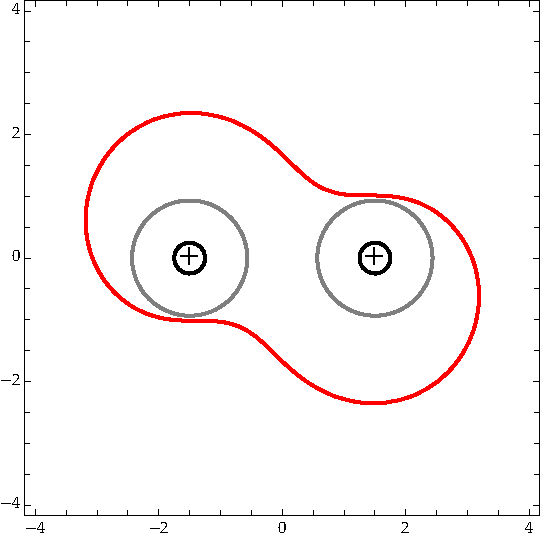
\includegraphics[width=\linewidth]{img/penrose_binaries/sks_regions.pdf}
  \caption{Regions of interest in the $t=0$ \ac{SKS} metric. The red region marks the boundary of the local ergosphere while the gray and black regions mark, respectively, the event horizons and singularities. The black crosshairs mark the centers of the black holes. The spacetimes parameters were chosen to be $M^{(1)} = M^{(2)} = 1/2$, $a^{(1)} = a^{(2)} = 1/4$ and $b = 3$}
  \label{fig:sks_ergo_plot}
\end{figure}

\subsubsection{Example 1}
\label{ch:sks_example_1}

For our first example, we have chosen the system parameters as $M^{(1)} = M^{(2)} = 1/2$, $a^{(1)} = a^{(2)} = 0.49$ and $b = 10$. The break-up point was chosen at coordinates $X^i = (6.3, 0, 0)$ and the background sphere radius was chosen to be $1.0 \times 10^6$. Following the same template of Table~\ref{tab:arbitrary_penrose_kerr_example_energy_mass}, Table~\ref{tab:arbitrary_penrose_sks_example_energy_mass} summarizes the initial energy and mass of the participating particles.

Once again, the first, second and third rows contain data relative to the entry, Penrose and exit orbits, respectively. The parameters for the entry and Penrose orbits are chosen explicitly, while the parameters of the exit orbit are computed via the conservation of 4-momentum at the break-point. The masses are explicitly chosen in order to satisfy Eq.~\eqref{eq:mass_constraint} and to provide a way of computing initial velocities via Eqs.~\eqref{eq:arbitrary_penrose_ellipse_parametric_1}-\eqref{eq:arbitrary_penrose_ellipse_parametric_2}
%
\begin{table}[]
  \centering
  \begin{tabular}{cc}
    \hline\hline
    $E(0)$                              & $m$                                 \\
    $1.0$                               & $1.0 \times 10^{-1}$                \\
    $8.0 \times 10^{-3}$                & $1.0 \times 10^{-4}$                \\
    $9.9199999999999999 \times 10^{-1}$ & $9.5800493929022838 \times 10^{-3}$ \\ \hline\hline
  \end{tabular}
  \caption{Initial energy and masses for the particles participating in the \ac{PP} example in the \ac{SKS} background.}
  \label{tab:arbitrary_penrose_sks_example_energy_mass}
\end{table}

Once more, following Table~\ref{tab:arbitrary_penrose_kerr_example_velocities}, Table~\ref{tab:arbitrary_penrose_sks_example_velocities} summarizes the initial velocities of the participating particles. Here, the values of the first two rows (representing the ingoing and Penrose trajectories, respectively), were computed via the parametrization described in the previous section together with data from Tab.~\ref{tab:arbitrary_penrose_kerr_example_energy_mass} while data on the third row, representing the outgoing particle, was computed via conservation of 4-momentum. The third column in this table shows the value of the ellipse parameter chosen for each orbit (except the exit orbit).
%
\begin{table}[]
  \centering
  \begin{tabular}{ccc}
    \hline\hline
    $V^x(0)$              & $V^y(0)$              & $\Theta$       \\
    $0.6769503786998466$  & $0.6740022058848380$  & $-25/200 \pi$  \\
    $0.5948571400034293$  & $-0.3343724878526367$ & $-100/200 \pi$ \\
    $0.66011565390809868$ & $0.68380243736284951$ & ---            \\ \hline\hline
  \end{tabular}
  \caption{Initial velocities for the particles participating in the \ac{PP} example in the \ac{SKS} background.}
  \label{tab:arbitrary_penrose_sks_example_velocities}
\end{table}

As Table~\ref{tab:arbitrary_penrose_kerr_example_results}, Table~\ref{tab:arbitrary_penrose_sks_example_results} summarizes the two energy measures (local and global on the first and second column, respectively) at the time when they hit the background sphere. The first row contains data relative to the ingoing orbit while the second contains data relative to the outgoing orbit. Note that $t_f$ does not necessarily coincide for the two orbits, since they might take arbitrarily long paths before escaping to infinity. The third column shows the absolute difference between global and local energies at the background sphere.
%
\begin{table}[]
  \centering
  \resizebox{\textwidth}{!}{
    \begin{tabular}{ccc}
      \hline\hline
      $E(t_f)$                            & $\varepsilon(t_f)$                  & $|E(t_f) - \varepsilon(t_f)|$       \\
      $2.4452985315377770 \times 10^{-1}$ & $2.4453006741751246 \times 10^{-1}$ & $2.1426373481014949 \times 10^{-7}$ \\
      $3.4638508542318119 \times 10^{-1}$ & $3.4638400572434974 \times 10^{-1}$ & $1.0796988314520917 \times 10^{-6}$ \\ \hline\hline
    \end{tabular}
  }
  \caption{Energy measures at the time of collision with the background sphere in the \ac{SKS} background}
  \label{tab:arbitrary_penrose_sks_example_results}
\end{table}

Finally, following Table~\ref{tab:arbitrary_penrose_kerr_example_efficiency}, Table~\ref{tab:arbitrary_penrose_sks_example_efficiency} summarizes the amount of energy extracted from the process in different forms. The first and second rows compute the difference between the energy of the outgoing and ingoing particles using different energy measures (local and global respectively). Since this difference is positive, we can conclude that energy was indeed extracted from the black hole. The last two rows compute the efficiency of the process for the two available energy measures, given by Eq~\eqref{eq:arbitrary_penrose_kerr_example_efficiency_formula}.
\begin{table}[]
  \centering
  \begin{tabular}{cc}
    \hline\hline
    $E_\text{out}(t_f)-E_\text{in}(t_f)$                     & $0.10185523226940352$ \\
    $\varepsilon_\text{out}(t_f)-\varepsilon_\text{in}(t_f)$ & $0.10185393830683726$ \\
    $\eta_E$                                                 & $0.41653495863897544$ \\
    $\eta_\varepsilon$                                       & $0.41652966700464295$ \\ \hline\hline
  \end{tabular}
  \caption{Energy difference and extraction efficiency of the process given different energy measures in the \ac{SKS} background.}
  \label{tab:arbitrary_penrose_sks_example_efficiency}
\end{table}

\subsubsection{Example 2}
\label{ch:sks_example_2}

In this example, we repeat the run detailed in Sec.~\ref{ch:sks_example_1} while changing the distance parameter from $b=10.0$ to $b = 7.21$. We have also changed the break-up point coordinates in each run so that it remains at $1.3$ coordinate distance units to the right of the right-most black hole. The results of this variation are summarized in Table~\ref{tab:arbitrary_penrose_sks_example_results_d_variation} where it is possible to see that the efficiency decreases as the black wholes get more distant from each other.

\begin{table}[]
  \centering
  \begin{tabular}{ccc}
    \hline\hline
    $d$  & $\eta_E$             & $\eta_\varepsilon$   \\
    10.0 & $0.4165349586389754$ & $0.4165293020302941$ \\
    9.69 & $0.4099912589653710$ & $0.4099855399919209$ \\
    9.38 & $0.4042822480170929$ & $0.4042767439403118$ \\
    9.07 & $0.3994849072973370$ & $0.3994792027270561$ \\
    8.76 & $0.3954568832639254$ & $0.3954513766173146$ \\
    8.45 & $0.3915618006432178$ & $0.3915564144708418$ \\
    8.14 & $0.3857189791093659$ & $0.3857135001267253$ \\
    7.83 & $0.3709406424619314$ & $0.3709350873643125$ \\
    7.52 & $0.3205512719659607$ & $0.3205458837844264$ \\
    7.21 & $0.1207168410527975$ & $0.1207122709189437$ \\ \hline\hline
  \end{tabular}
  \caption{Energy extraction efficiency for the configuration detailed in Sec~\ref{ch:sks_example_1} while varying the distance parameter $b$ and keeping the break-up point at $1.3$ coordinate distance unites to the right of the rightmost black hole in the \ac{SKS} background.}
  \label{tab:arbitrary_penrose_sks_example_results_d_variation}
\end{table}

\subsubsection{Example 3}
\label{ch:sks_example_3}

In this example we vary the mass of the left-most black hole $M^{(2)}$ from $0.5$ to $0.275$ while also changing the spin parameter according to $a^{(2)} = 0.98 M^{(2)}$. We keep fixed the mass $M^{(1)} = 0.5$, the spin parameter $a^{(1)} = 0.49$, the distance parameter $b=20.0$ and the break-up point $(11.0, 0.0, 0.0)$. This configuration is analogue to that of the single Kerr black hole example of Sec.~\ref{ch:kerr_example}. The results are summarized in Table~\ref{tab:arbitrary_penrose_sks_example_results_M2_variation}, where it is possible to see that as the mass of the companion black hole decreases, the extraction efficiency decreases.

\begin{table}[]
  \centering
  \begin{tabular}{ccc}
    \hline\hline
    $M2$  & $\eta_E$             & $\eta_\varepsilon$   \\
    0.500 & $0.1057279994029897$ & $0.1057236710602922$ \\
    0.475 & $0.0870377969920106$ & $0.0870336429442202$ \\
    0.450 & $0.0712047949044382$ & $0.0712008663973118$ \\
    0.425 & $0.0578255784926676$ & $0.0578218053066227$ \\
    0.400 & $0.0465203386664686$ & $0.0465166569217887$ \\
    0.375 & $0.0369572283763885$ & $0.0369537431441037$ \\
    0.350 & $0.0288551456052595$ & $0.0288518045002344$ \\
    0.325 & $0.0219792546154663$ & $0.0219759777138235$ \\
    0.300 & $0.0161341223097530$ & $0.0161310745614111$ \\
    0.275 & $0.0111575173287062$ & $0.0111545996429916$ \\ \hline\hline
  \end{tabular}
  \caption{Energy extraction efficiency for fixed mass $M^{(1)} = 0.5$, spin parameter $a^{(1)} = 0.49$, distance parameter $b=20.0$ and break-up point $(11.0, 0.0, 0.0)$ and varying Mass $M^{(2)}$ and spin parameter $a^{(2)} = 0.98 M^{(2)}$.}
  \label{tab:arbitrary_penrose_sks_example_results_M2_variation}
\end{table}